\chapter{\babDua}
Membuat desain sebuah perangkat IC membutuhkan proses yang panjang dan sumberdaya manusia yang banyak, serta tingkat ketelitian yang tinggi. Oleh karenanya di butuhkan biaya yang tidak kecil dan waktu yang cukup lama hanya untuk membuat sebuah desain IC. Dengan kerumitan yang tinggi serta waktu yang lama dalam setiap prosesnya kadang pihak yang tak bertanggung jawab melakukan kecurangna dengan mecuri desain untuk memotong waktu dan biaya yang di butuhkan utuk produksi. sehingga menjadi masalah dalam dunia permanufakturan ic. \cite{Azriel2017}

\section{Very Large Scale Integration}
\textit{Very Large Scale Integration} atau disingkat LSI merupakan proses pembuatan sebuah IC dengan mengkombinasikan ribuan transistor ke dalam sebuah chip. VLSI ada sejak tahun 1970-an ketika semikonduktor kompleks dan teknologi komunikasi sedang berkembang. Mikroprosesor merupakan salah satu peraangkat VLSI. Sebelum adanya teknologi VLSI kebanyakan IC memiliki set fungsi yang terbatas yang dapat di jalankan. Sebuah perangkat chip elektronik dahulu hanya fokus pada sebuah fungsi seperti CPU, ROM, RAM dan rangkaian logika lainnya. Dengan adanya VLSI memungkinkan disainer IC untuk menambahkan berbagai fungsi kedalam sebuah chip IC. \cite{vlsi.hist} 

\subsection{Arus Pengembangan LSI}
Integrated Circuit (IC) merupakan teknologi sirkuit elektronika yang lebih maju. Sebuah rangkaian elektronika dibuat dari berbagai komponen elektronika yang berbeda beda seperti transistor, resistor, kapasitor dan dioda yang saling tersambung satu sama lain. \cite{vlsi.hist}

Transistor merupakan komponen terpenting pada pengembangan teknologi komputer moderen. Sebelum ditemukannya transistor. Para Engineer harus menggunakan tabung vakum. Tabung vakum dapat bekerja sebagai saklar elektronik. Namun tabung vakum membutuhkan daya dan ruang yang besar, mahal, serta kemampuan eksekusi yang lambat membuat tabung vakum tergantikan oleh transistor.

Dengan ditemukannya transistor yang ukuran dan kebutuhan dayanya yang kecil namun tetap efektif, Para Engineer elektronik di tahun 1950an melihat banyak sekali kemungkinan untuk implementasinya pada rangkaian elektronik yang lebih maju. Dengan semakin meningkatnya kompleksitas pada rangkaian elektronik munculah masalah-masalah baru.

Salah satunya adalah ukuran rangkaian. Sebuah rangkaian kompleks seperti komputer sangat bergantung pada kecepatan. Apabila jumlah komponen pada komputer terlalu banyak maka sambungan antar komponen juga semakin banyak dan semakin panjang, sehingga menyebabkan kecepatan transfer sinyal listrik menjadi berkurang yang menyebabkan proses pada komputer menjadi lambat.

Tahun 1958 masalah ini dapat dipecahkan oleh ide Jack S Kilby yang idenya adalah merangkai komponen elektronika dalam sebuah blok silikon (Monolithic Idea). Idenya tersebut tidak hanya mengurangi ukuran rangkaian namun juga mengurangi kebutuhan kabel sambungan antar rangkaian serta manufakturingnya dapat diautomasi. Akan tetapi idenya tersebut masih memiliki banyak masalah lain. Walaupun begitu, idenya tersebut mendapatkan penghargaan nobel di tahun 2000.

Setengah tahun setelah Kilby mencetuskan idenya tentang rangkaian Monolithic. Robert Noyce memiliki jawaban untuk beberapa permasalahan pada ide Kilby. Yaitu interkoneksi antar rangkaian. Yaitu menambahkan lapisan metal pada lapisan terakhir dan menghilangkan sebagian lapisannya sehingga sambungan antar komponen dapat terbentuk.

\begin{figure}
	\centering
	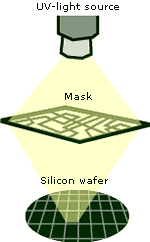
\includegraphics[width=0.35\textwidth]
	{pics/steping.png}
	\caption{Produksi Chip Moderen}
	\label{fig:produksiChipModeren}
\end{figure}

Chip pada zaman sekarang berbasis pada photolithography. Pada teknik ini digunakan radiasi sinar Ultra Violet yang melewati sebuah mask menuju lembaran silikon yang di lapisi filem photosensitive untuk membentuk suatu rangkaian.

\subsection{Kemungkinan Serangan Desain LSI}
Dilihat dari proses developing, terdapat 2 cara untuk mendapatkan sebuah desain untuk di kloning. Pertama dengan mengambil langsung data mentah desain atau "blueprint" dan Reverse Engineering saat barang telah dipublikasi di pasaran.

\begin{figure}
	\centering
	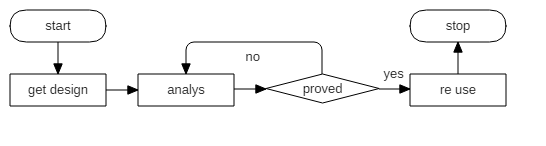
\includegraphics[width=1.05\textwidth]
	{diagrams/untrustSource.png}
	\caption{Clonning/Sumber Tidak Terpercaya}
	\label{fig:untrustsource}
\end{figure}

Dalam segi ini serangan dilakukan dengan cara mencuri langsung desain yang sudah siap di fabrikasi serta uji coba kebenaran. Bila pencuri mendapatkan desain yang telah di uji coba, maka pencuri tinggal langsung memperbanyak desain yang telah di curi.

\begin{figure}
	\centering
	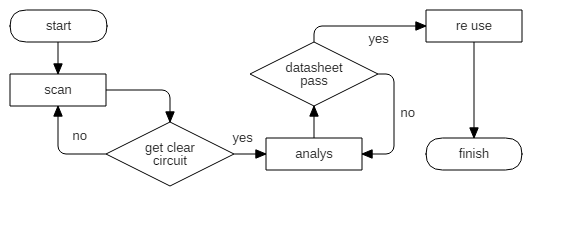
\includegraphics[width=1.05\textwidth]
	{diagrams/reverseEngineering.png}
	\caption{RE (Reverse Engineering)}
	\label{fig:reverseengineering}
\end{figure}

Untuk serangan jenis ini, pencuri sudah pendapatkan produk dari pasar yang telah teruji, pencuri tinggal melakukan scan rangkaian kemudian mengujinya dengan datasheet. Apabila hasil scan desain produk di dapati rangkaian yang konkrit/jelas dan rangkaian tersebut telah teruji sesuai datasheet. Maka pencuri tinggal melakukan fabrikasi.

\subsection{Mengatasi Serangan terhadap Desain LSI}
Dengan meninjau kemungkinan dari tipe serangan, terdapat berbagai cara untuk mengatasi setiap serangan serangan tersebut. Dari reverse engineering hingga untrust source. untuk reverse enginering digunakan teknik anti reverse engineering dan untuk untrust source digunakan teknik identifier dan dengan enclosure agreement law.

\begin{figure}
	\centering
	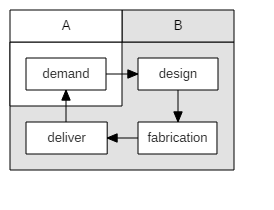
\includegraphics[width=0.5\textwidth]
	{diagrams/oldBusinessLSI.png}
	\caption{Model Bisnis Lama}
	\label{fig:oldbiss}
\end{figure}

Pada model gambar diatas, kegiatan desain, fabrikasi dan deliveri di lakukan oleh satu pihak yang sama. Proses pembuatan suatu perangkat IC dimonopoli oleh 1 perusahaan. Sehingga kemungkinan serangan hanya ada di antara pihak A dan Pihak B.

\begin{figure}
	\centering
	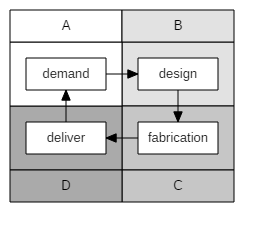
\includegraphics[width=0.5\textwidth]
	{diagrams/newBusinessLSI.png}
	\caption{Model Bisnis Baru}
	\label{fig:newbiss}
\end{figure}

Namun seiring dengan perkembangnya jaman. Monopoli proses dari desain, fabrikasi hingga deliveri mulai sulit di terapkan. Karena dengan semakin berkembangnya jaman dan deman akan fitur desain semakin tinggi, otomatis biaya semakin tinggi dan kompleksitas suatu desain semakin rumit serta waktu untuk menyelesaikan suatu desain semakin lama.

Oleh karena itu sekarang mulai diterapkan Fabless manufakturing atau joint venture untuk membuat suat perangkat elektronika. Setidaknya pada proses bisnis ini terdapat 4 pihak. Pihak A dari keinginan pasar, pihak B yang melakukan perancangan desain, pihak C yang elakukan fabrikasi hasil rancangan pihak B dan Pihak D yang melakukan deliveri hasil fabrikasi di pihak C ke A.

\section{Teknik Proteksi}
Dari berbagai teknik yang telah digunakan, penulis melakukan penggabungan 2 teknik pengamanan dalam sebuah desain IC. Dalam penelitian ini dilakukan penggabungan 2 teknik agar cakupan wilayah keamanan sebuah IC semakin luas. Berikut teknik yang digabungkan dalam penelitian kali ini.

\subsection{Digital Signal Processing Filter}
Digital Signal Prosesing (DSP) merupakan pengolahan sinyal digital, seperti digunakan pada komputer hingga untuk melakukan berbagai operasi proses sinyal. Sinyal yang diproses merupakan kumbulan bilangan sekuensial yang merepresentasikan sampel dari variabel sinyal kontinyu pada suatu domain seperti domain waktu, ruang atau frekuensi.

Pada pengolahan sinyal, sebuah filter adalah sebuah alat atau proses yang menghilangkan beberapa komponen atau fitur yang tidak di inginkan dari suatu sinyal. Filtering merupakan kelas proses sinyal, 

\subsection{Polimorphisme Gate}
Polimorphisme Gate merupakan teknik pengecoh yang di gunakan dalam perlindungan desain IC. Sebagai contoh sebuah rangkaian dengan ouput F dan input A,B dan C akan memiliki hasil yang berbeda jika parameters k yang diberikan berbeda. Misal bila parameter k diisi dengan kombinasi 0101 maka outputnya adalah
\begin{center}
	F = A XOR (A \textbf{AND} B)
\end{center}
Sedangkan bila parameter k diisi dengan kombinasi 1101 maka outputnya menjadi
\begin{center}
	F = A XOR (A \textbf{NOR} B)
\end{center}

\begin{figure}
	\centering
	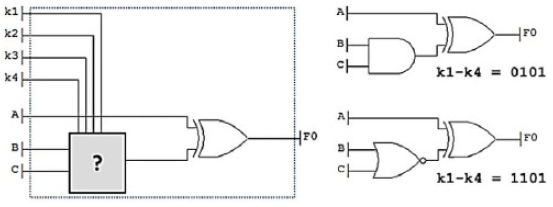
\includegraphics[width=0.75\textwidth]
	{pics/polymorphgate.png}
	\caption{Polymorph gate}
	\label{fig:poly}
\end{figure}

\section{Peralatan dan Teknologi}
Dalam penelitian kali ini dibutuhkan beberapa peralatan dan standard teknologi untuk mengembangkan teknik perlindungan intelektual properti. Sebagai penunjang dalam pembuatan perlindungan, penulis menggunakan tools dan teknologi yang umum digunakan dalam proses pengembangan desain LSI.

\subsection{Verilog HDL}
Verilog HDL merupakan bahasa pendeskripsi hardware yang digunakan untuk mendesain dan dokumentasi sistem elektronika. Verilog HDL memungkinkan perancang mendesain pada berbagai tingkatan abstraksi.

Verilog HDL berasal dari Automated Integrated Design System (yang kemudian berubah nama menjadi Gateway Design Automation) pada tahun 1985. Saat itu perusahaan tersebut dipegang oleh Dr. Prabhu Goel, pendiri PODEM test generation algorithm. Verilog HDL di desain oleh Phil Moorby, yang kemudian menjadi chief Designer untuk Verilog-XL dan perusahaan rekan pertama di Cadance Design System. 

Awalnya Verilog dibuat sebagai bahasa simulasi. Kemudian setelah berkembang tidak hanya digunakan untuk simulasi namun juga untuk sintesis. (source www.verilog.com)

\subsection{Yosys Open SYnthesis Suite}
Yosys adalah sebuah framework untuk sintesis Verilog RTL. Sekarang ini memiliki suport yang extensif pada Verilog-2005 dan mendukun berbagai set basik algoritma sintesis untuk berbagai domain aplikasi.

\begin{figure}
	\centering
	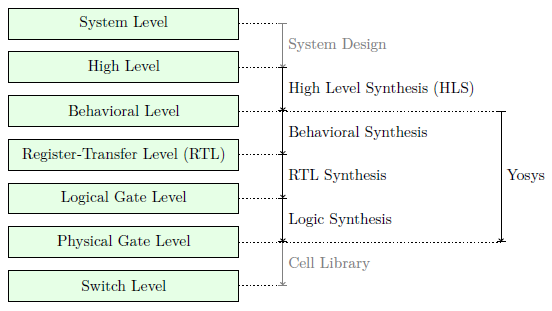
\includegraphics[width=0.75\textwidth]
	{pics/yosys.png}
	\caption{Perbedaan Tinkatan Abstraksi dan Sintesis Yosys}
	\label{yosys}
\end{figure}

\subsection{Xilinx ISE Design Suit}
Xilinx ISE Design Suit merupakan Computer Aided Design (CAD) keluaran Xilinx yang digunakan untuk developing IC.

\begin{figure}
	\centering
	
\includegraphics[width=0.4\textwidth]
	{pics/ise-logo.jpg}
	\caption{Logo Xilinx ISE Design Suit}
	\label{ise}
\end{figure}

\subsection{FPGA Elbert V2 Board}
FPGA merupakan kepanjangan dari Field Programmable Gate Array adalah perangkat keras yang biasa digunakan dalam proses manufakturing IC. FPGA digunakan untuk mensimulasikan draft rancangan IC yang siap untuk di test yang apabila telah lolos test akan di lanjutkan ke tahap layout. FPGA hanya digunakan apabila rancangan membutuhkan input dari perangkat lain atau program kernel.

\begin{figure}
	\centering
	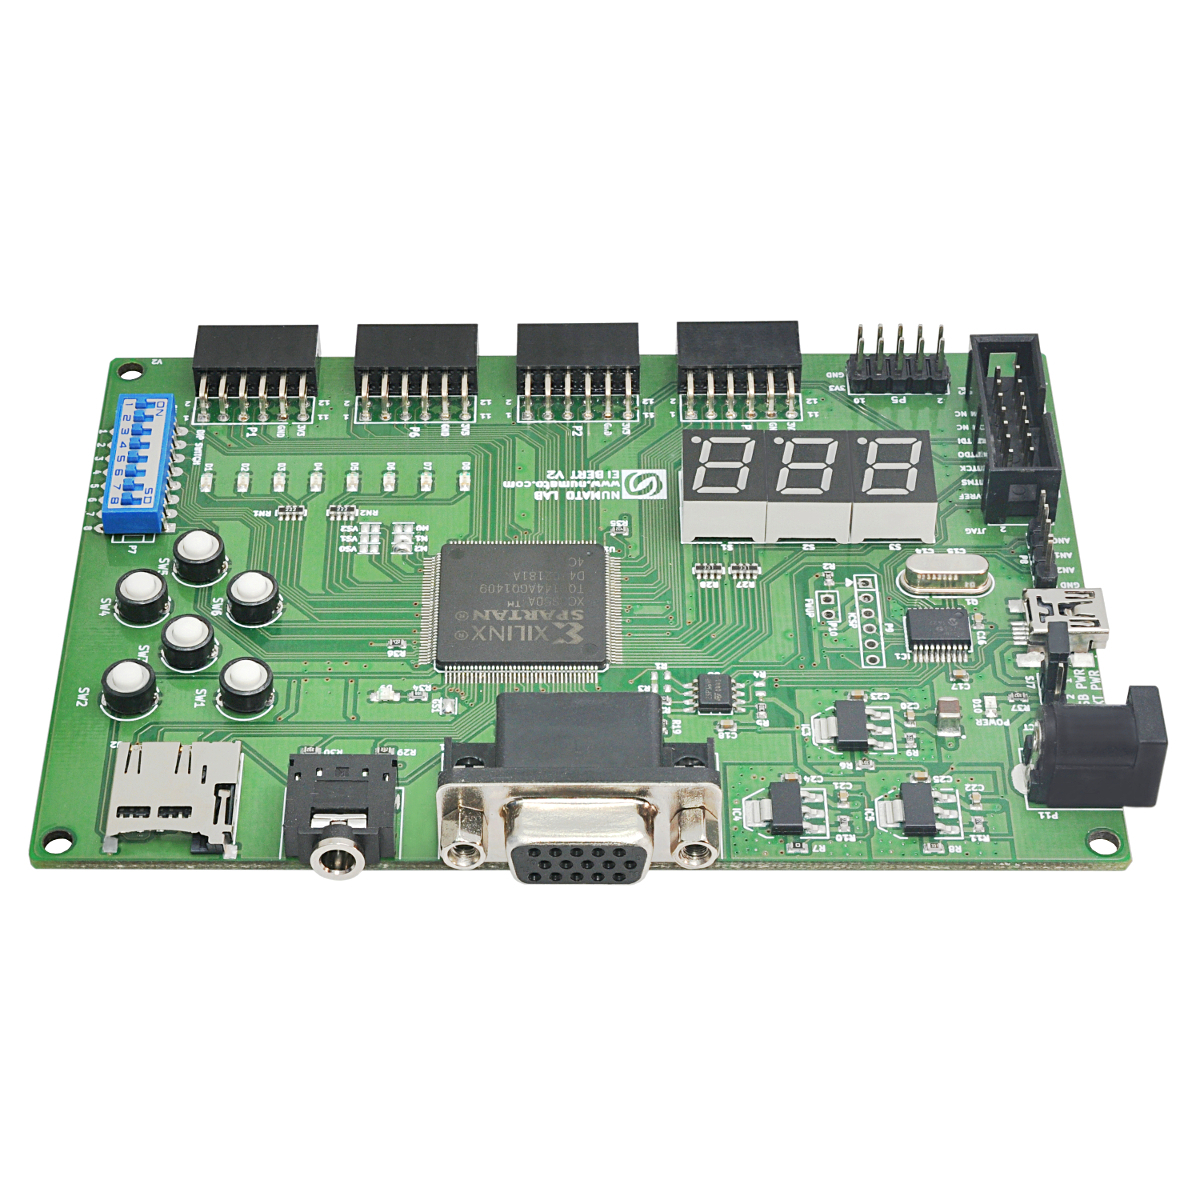
\includegraphics[width=0.75\textwidth]
	{pics/elbertv2.jpg}
	\caption{FPGA Board - Elbert V2}
	\label{fig:fpga}
\end{figure}

Elbert V2 merupakan Board yang simple namun serbaguna untuk pembelajaran atau pengembangan. Board ini menggunakan Xilinx Spartan 3A FPGA. Pada Development Board ini memiliki fitur FPGA dari Xilinx XC3S50A dengan 144 pin dengan maksimum 108 user IO. Dilengkapi dengan antarmuka USB2 untuk kemudahan konfigurasi ke SPI flash. 

\section{Target IP Core}
Watermark adalah rangkaian yang tidak boleh berdiri sendiri pada implementasinya walaupun dalam pengembangannya bisa di lakukan mandiri. Dalam penelitian kali ini Module yang akan di watermark adalah modul ALU.

\subsection{Aritmatic Logic Unit (ALU)}
Aritmatik Logic Unit (ALU) adalah kombinasi rangkaian elektronik digital yang melakukan fungsi aritmatika dan operasi bitwise pada bilangan integer binari. Ini sangat kontras dengan Floating Point Unit (FPU), yang melakukan operasi bilangan floating point. Sebuah ALU pada dasarnya bagian dari berbagai macam blok rangkaian komputasi, termasuk Central Prosesing Unit (CPU). Sebuah CPU, FPU, atau GPU mungkin memiliki banyak ALU di dalamnya.

\begin{figure}
	\centering
	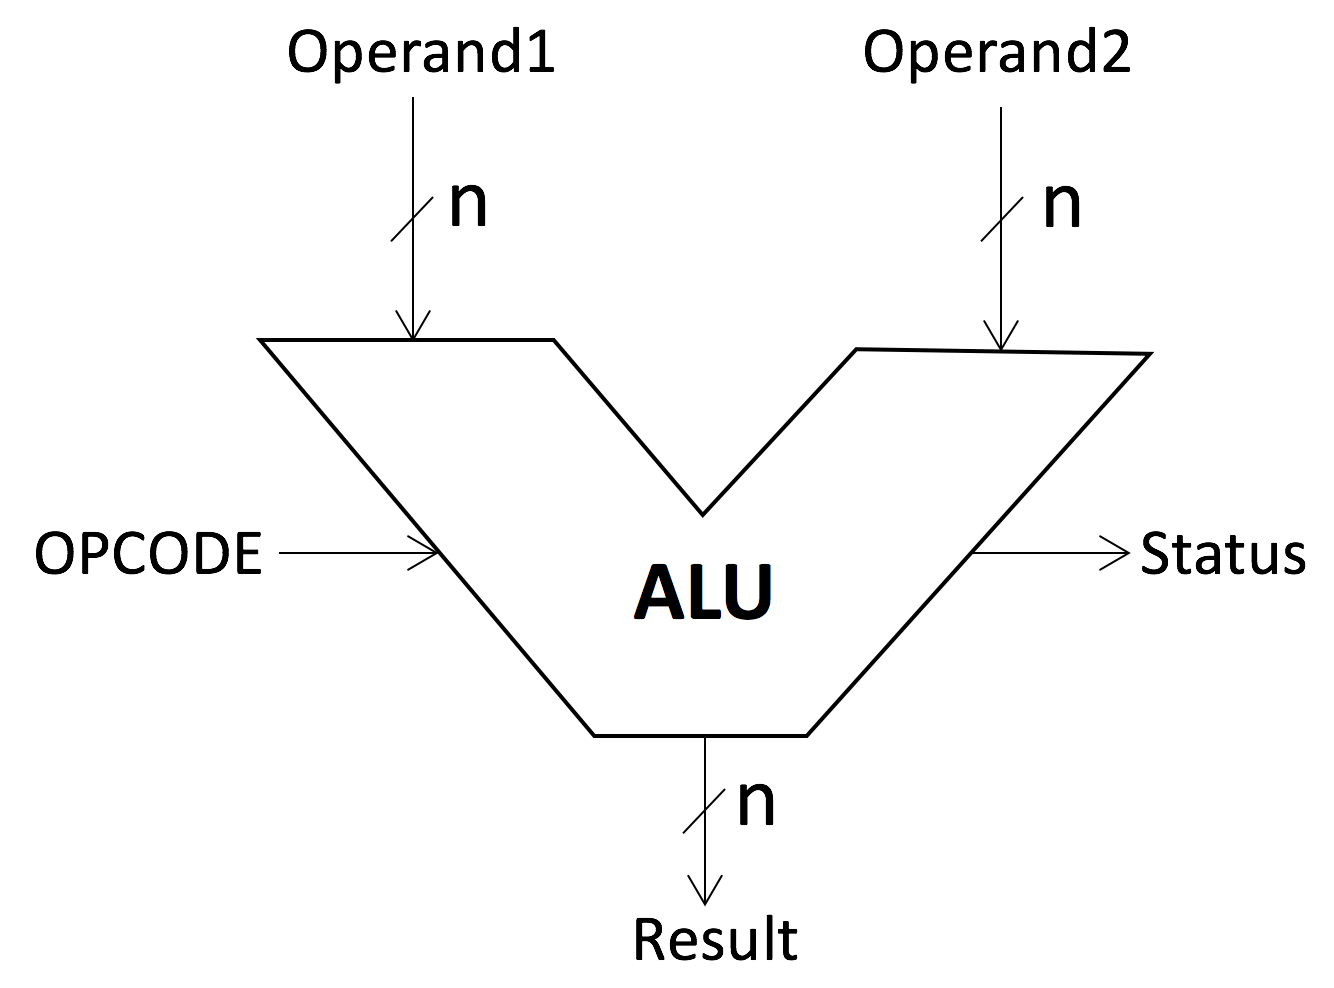
\includegraphics[width=0.5\textwidth]
	{pics/alu.png}
	\caption{ALU}
	\label{alu}
\end{figure}

